% Matteo Esposito
% Corso di Ingegenria degli Algoritimi
% Dicembre 2017
% Main.tex

%--------------- Package Usati ---------------%
\documentclass[10pt,a4paper,oneside]{matc3mem}
\usepackage{geometry}
\geometry{
	a4paper,
	total={170mm,257mm},
	left=10  mm,
	top=20mm,
	right=10 mm,
}
\usepackage{tikz}
\usepackage{multicol} 
\usepackage[utf8]{inputenc}
\usepackage{graphicx}
\usepackage{listings,lstautogobble}
\usepackage{xcolor}
\usepackage{graphicx}
\usepackage{wrapfig}
\usepackage[ampersand]{easylist}
\usepackage{float}
\usepackage[italian]{babel}
\usetikzlibrary{calc}

\definecolor{RoyalBlue}{cmyk}{1, 0.50, 0, 0}

\lstset{language=Python,
	keywordstyle=\color{RoyalBlue},
	basicstyle=\scriptsize\ttfamily,
	commentstyle=\ttfamily\itshape\color{gray},
	stringstyle=\ttfamily,
	showstringspaces=false,
	breaklines=true,
	frameround=ffff,
	frame=single,
	rulecolor=\color{black},
	autogobble=true
}
\usepackage{showexpl}
\usepackage{zlmtt}
\usepackage{fancyvrb}
\usepackage{ragged2e}
\usepackage{titling}
\usepackage{alltt}
%----------------------------------------------%


\begin{document}

%--------------- Trick Usati ---------------%
\renewcommand\maketitlehooka{\null\mbox{}\vfill}
\renewcommand\maketitlehookd{\vfill\null}
%------------------------------------------%

%--------------- Titolo ---------------%
\author{Matteo Esposito \\ Matricola: 0238638}
\title{Relazione Progetto in Itinere II \\
	\large Corso di Ingegneria Degli Algoritmi}
\date{Gennaio 2018}
%-------------------------------------%

%--------------- Comandi Iniziali---------------%
\frontmatter
\begin{titlingpage}
\maketitle
\end{titlingpage}
\newpage
\tableofcontents
%----------------------------------------------%

%--------------- Capitoli ---------------%
\mainmatter
\chapter{Abstract}
\section{Premessa}
L'algoritmo presentato vorrebbe tentare di risolvere il problema N.2 il quale chiedeva:\\ 
\begin{center}
	\emph{"Sia dato un grafo non orientato e non pesato  G . Data una coppia di nodi ($n_1,n_2$)  in  G , la distanza dist($n_1,n_2$)  \'e il minor numero di archi necessari a connettere  $n_1$  e  $n_2$. Un nodo  \'e  medio di $n_1$ ed $n_2$ se e solo se \'e equidistante da $n_1$ e  $ n_2$,  ovvero se $dist(n_1,m)$=  $dist(m,n_2)$ . Progettare e implementare un algoritmo che, dato un grafo non orientato e non pesato  G , determini il nodo m  *  che risulta essere  medio per il maggior numero di coppie di nodi ."}\\
\end{center}
L'approccio risolutivo consta dell'utilizzo di operazioni pre-esistenti, forniteci attraverso le classi e gli snipset presenti sulla pagina di GitHub del Corso, con una classe "GraphExtended" che riporta alcune funzioni il cui scopo \'e estendere ulteriormente la classe GraphIncidenceList. Il tempo di esecuzione totale nel caso peggiore risulta essere $O(|V|*|E|)$ in quanto l'algoritmo scelto per risolvere il problema consta efettivamente di due loop principali nel quale scandendo il singolo nodo scandisce tutti gli archi del grafo.
L'Algoritmo scelto per la risoluzione era un algoritmo pre-esistente frutto della ricerca accademica del prof. Ulrich Brandes della università di Konstanz in Germania, esso nacque per velocizzare la catalogazione dei nodi di un grafo per i rispettivi indici di "Betweennes Centrality". La mia implementazione, nata dallo pseudo-codice presente all'interno del Paper Accademico di Brandes, ha un differente approccio nella gestione del risultato in quanto, mentre lo scopo dell'originale era restituire semplicemente il dizionario, attraverso operazioni più o meno costanti, ho voluto far restituire all'algoritmo una tripla di elementi così costituita: \\
\begin{easylist}[itemize]
	& int: massimo indice di Betweennes Centrality
	& set: tutti i nodi che condividono il massimo indice di Betweennes Centrality
	& Dizionario:	
	&& Chiave: ID Nodo
	&& Valore: Indice di Betweennes Centrality del nodo \\ \\
\end{easylist} 

Il codice \'e cos\'i strutturato:
\begin{easylist}[itemize]
	& main.py: contenente essenzialmente le DEMO dell'algoritmo
	& la classe "ProjUtilities":contenente le funzioni principali per la genrazione pseudo-randomica dei grafi
	& brandes.py: core del progetto contenente l'implementazione in python dello pseudo-codice del prof. Brandes
	& la succitata classe GraphExtended contenente uno dei core dell'algoritmo stesso \\( la funzione \emph{convertToBradesGraphAlgo()} )
	& tutte le librerie e classi fornite precedentemente attraverso la pagina di GitHub.
\end{easylist} 


\chapter{Richiami Teorici}
\section{Criterio di Bellman}
\begin{center}
	\emph{"Un vertice $v \in V$ giace su un cammino minimo tra i vertici $s,t \in V$ ( \'e centrale nel loro cammino minimo),\\ se e solo se $dist(s,t)=dist(s,v)+dist(v,t)$}\\
\end{center}

\section{Betweennes Centrality}
Nella teoria dei grafi, la \emph{Betweennes Centrality} è una misura della centralità in un grafo basata su cammini minimi. Per ogni coppia di vertici in un grafo connesso, esiste almeno un cammino minimo tra i vertici in modo tale che o il numero degli archi attraversati dal percorso (per i grafi non pesati) o la somma dei pesi dei bordi (per i grafi pesati ) è ridotto al minimo. La \emph{Betweennes Centrality}  per ciascun vertice è il numero di questi cammini minimi che attraversano il vertice.

\section{Dipendeza tra nodi}
Sia $G=(V,E)$ un \emph{grafo} e siano $s$,$t$ una coppia fissa di nodi del \emph{grafo}. Sia $\delta_{st} $ il numero di cammini minnimi tra $s$ e $t$ e sia $\delta_{sv}(V)$ il numero di cammini minimi che passano per $v$. Definiamo allora \emph{dipendenza} di un nodo sorgente $s$ su di un vertice $v$ come segue: \\
		$$
			\delta_s(v) = \sum_{t \in V}^{} \frac{\delta_{st}(v)}{\delta_{st}}
 		$$


\noindent \\ \\ Quanto precede riesce a catturare l'importanza di un nodo $v$ rispetto ad un nodo $s$ e $t$. La Betweennes Centrality di un vertice $v$ allora si può definire come:

$$
	BC(v) = \sum_{s\neq v \in V} \delta_s(v)
$$

\noindent \\ \\ L'intuizione di Brandes, partendo da questa relazione, fu proprio rendersi conto che la dipendenza del nodo $v$ soddisfi in realtà la seguente ricorrenza:\\
$$
	\delta_s(v) = \sum_{w:v \in pred(s,w)} \frac{\delta_{sv}}{\delta_{sw}}(1 + \delta_s(w))
$$ 
\noindent	\\ Con \emph{pred(s,v)} l'insieme dei predecessori di $w$ nel cammino minimo da $s$ a $w$.
\chapter{L'Algoritmo}
\paragraph{Attenzione:} di seguito verrà analizzato l'algoritmo di Brandes nella sua versione pura ed originale tralasciando le mie personali modifiche comunque commentate nel codice sorgente ed ininfluenti da un punto di vista di Complessità Temporale.

\section{Fase Preliminare ( SOLO VERSIONE DEMO )}
$\mathbf{Tempo: O(n^2)}$\\ 	\\
Nella fase preliminare l'algoritmo crea un grafo, in maniera pseudo-randomica, attraverso i metodi \emph{generateAcycleGraph()} o  \emph{generateCyclicGraph()} ( contenuti in ProjUtilities).
Il presente metodo, per quanto veloce possa essere il tempo di esecuzione è pari ad un O($n^2$). Chiaramente \'e un metodo esistente solo nella DEMO dell'algoritmo mentre la sua implementazione pura non prevede affatto questa parte ragion per cui nel calcolo totale ho ignorato tale risultato.
\newline
\newline

% Albero A
\paragraph{Grafo Generato Aciclico:}
\begin{center}
	\begin{tikzpicture}[->,>=,shorten >=1pt,auto,node distance=3cm, thick,main node/.style={circle,draw,font=\sffamily\Large\bfseries}]
	
	\node[main node] (8) [yshift=.88 cm]{8};
	\node[main node] (0) [below of =8] {0};
	\node[main node] (1) [below of=0] {1};
	\node[main node] (2) [left of=8] {2};
	\node[main node] (4) [right of=8] {4};
	\node[main node] (3) [below  of=4] {3};
	\node[main node] (5) [right of=4] {5};
	\node[main node] (6) [below of=2] {6};
	\node[main node] (7) [left of=2] {7};
	\node[main node] (9) [below left of=7] {9};
	\node[main node] (27) [above left of=7] {27};

	\node[main node] (10) [above right of=5] {10};
	\node[main node] (11) [below right of=5] {11};
	\node[main node] (12) [below left of=1] {12};
	\node[main node] (13) [below right of=1] {13};
	\node[main node] (14) [above of=4] {14};
	\node[main node] (15) [right of=14] {15};
	\node[main node] (16) [above right of=15] {16};
	\node[main node] (17) [below right of=15] {17};
	
	\node[main node] (18) [above of=2] {18};
	\node[main node] (19) [right of=18] {19};
	\node[main node] (20) [left of=18] {20};
	\node[main node] (21) [above left of=19] {21};
	\node[main node] (22) [above left of=20] {22};
	\node[main node] (23) [above of=19] {23};
	\node[main node] (24) [above of=20] {24};
	\node[main node] (25) [above right of=19] {25};
	\node[main node] (26) [left of=20] {26};
 	%\coordinate (8) at ($(1)!0.5!(3)$) {8};

	\path[every node/.style={font=\sffamily\small}]
		(0) 
		edge node [] {} (1)

		(1)
		edge node [left] {} (12)
		edge node [left] {} (13)
		
		(2) 
		edge node [right] {} (8)
		edge node {} (7)
		edge node [below] {} (6)
		
		(3) 

		
		(4) 
		edge node [left] {} (3)
		edge node [right]   {} (5)
		edge node [above]	{} (14)
		
		(5)
		edge node [right] {} (10)
		edge node [right] {} (11)
		
		(7)
		edge node [left] {}(9)
		edge node [left] {}(27)
		
		(8) 
		edge node [right]	{} (4)
		edge node [below] {} (0)
		
		(15)
		edge node [right]	{} (16)
		edge node [right]	{} (17)
		edge node [left]	{} (14)
		
		(18)
		edge node [below]	{} (2)
		edge node [right]	{} (19)
		edge node [left]	{} (20)
		
		(19)
		edge node [left]	{} (21)
		edge node [above]	{} (23)
		edge node [right]	{} (25)
		
		(20)
		edge node [above left]	{} (22)
		edge node [above]	{} (24)
		edge node [left]	{} (26)
		;
		      
		

	\end{tikzpicture}
	
	
	%/*%
	%  edge [loop right] node {0.6} (4)
	%edge [bend right] node[right] {0.2} (1);
	%*/
\end{center}

% Albero B
\paragraph{\newline Grafo Generato Ciclico \newline}
\begin{center}
	\begin{tikzpicture}[->,>=,shorten >=1pt,auto,node distance=3cm, thick,main node/.style={circle,draw,font=\sffamily\Large\bfseries}]
	
	\node[main node] (0) {0};
	\node[main node] (1) [below of=0] {1};
	\node[main node] (2) [below left of=1] {2};
	\node[main node] (3) [below right of=2] {3};
	\node[main node] (4) [below right of=1] {4};
	\node[main node] (5) [right of=4] {5};
	\node[main node] (6) [below of=3] {6};
	\node[main node] (7) [left of=2] {7};
	\node[main node] (8) [below of=1, yshift=.88 cm]{8};
 	%\coordinate (8) at ($(1)!0.5!(3)$) {8};
	
	\path[every node/.style={font=\sffamily\small}]
		(0) edge node [] {} (1)
			  edge [bend left] node[] {} (5)
			
		(1)	edge node [left] {} (4)
			 edge node [below] {} (8)
		(2) edge node [right] {} (1)
		edge node {} (8)
		edge node {} (7)
		(3) edge node [right] {} (2)
			  edge node [below] {} (6)
			  edge node [above] {} (8)
		(4) edge node [left] {} (3)
		      edge node [right] {} (5)
		      edge node [left] {} (8)
		      
		 (6) edge [bend left] node [] {} (7);
		

	\end{tikzpicture}
	
	
	%/*%
	%  edge [loop right] node {0.6} (4)
	%edge [bend right] node[right] {0.2} (1);
	%*/
\end{center}

\paragraph{Attenzione:} per ragioni di DEBUG o di TESTING fornisco di seguito l'Array ed il Dizionario dei due grafi di cui sopra per permetterne la verifica dei risultati. \newline \newline
%\emph{Grafo Aciclico: \\}
%V = [ ] \\
%A = \{\}
%\newline 
%\newline
%\emph{\\ \\ Grafo Ciclico: \\}
%V = [ ] \\
%A = \{\}

\emph{ \\Grafo Aciclico: \\ \\}
V = [ 0, 1, 2, 3, 4, 5, 6, 7, 8, 9, 10, 11, 12, 13, 14, 15, 16, 17, 18, 19, 20, 21, 22, 23, 24, 25, 26, 27 ]
\\ \\
A = \{ 0:[1, 8],  1:[0, 12, 13], 2:[7, 18, 8, 6], 3:[4], 4:[8, 14, 5, 3], 5:[4, 10, 11], 6:[2], 7:[27, 2, 9], 8:[2, 4, 0], 9:[7], 10:[5], 11:[5], 12:[1], 13:[1], 14:[4, 15], 15:[14, 16, 17], 16:[15], 17:[15], 18:[20, 19, 2], 19:[18, 21, 23, 25], 20:[26, 22, 24, 18], 21:[19], 22:[20], 23:[19], 24:[20], 25:[19], 26:[20], 27:[7]\}
\\ \\
R: (442.0, \{2\}, \{0: 144.0, 1: 102.0, 2: 442.0, 3: 0, 4: 342.0, 5: 102.0, 6: 0, 7: 102.0, 8: 436.0, 9: 0, 10: 0, 11: 0, 12: 0, 13: 0, 14: 144.0, 15: 102.0, 16: 0, 17: 0, 18: 336.0, 19: 150.0, 20: 150.0, 21: 0, 22: 0, 23: 0, 24: 0, 25: 0, 26: 0, 27: 0\})


\emph{\\ \\ Grafo Ciclico: \\ \\}
V = [0, 1, 2, 3, 4, 5, 6, 7, 8]
\\ \\
A = \{ 0:[1, 5], 1:[2, 0, 4, 8], 2:[7, 1, 8, 3], 3:[2, 8, 4, 6], 4:[8, 1, 5, 3], 5:[4, 0], 6:[7, 3], 7:[2, 6], 8:[2, 1, 4, 3] \}
\\ \\
R: (17.06666666666667, \{1\}, \{0: 1.9, 1: 17.06666666666667, 2: 17.066666666666666, 3: 17.066666666666666, 4: 17.066666666666666, 5: 1.9, 6: 1.9, 7: 1.9, 8: 4.133333333333334\})
\\
\noindent 
\paragraph{Attenzione:}Come si può evincere dalla quantità di dati e dal Return dell'algoritmo, a grafi complessi corrispondo valori di Betweennes Centrality più complessi e più raffinati, al fine di semplificarne l'analisi è ovviamente implementabile la \emph{normalizzazione} dei dati come è già di per se fatto all'interno di librerie come la NetworkX ( Python ).


\newpage

\section{Inizializzazione}
$\mathbf{Tempo: O(n)}$\\ 	\\
L'inizializzazione dell'algoritmo consta di alcuni allocamenti preventivi di spazio in memoria, procede quindi ad inizializzare da subito il dizionario "C" ponendo a zero tutti i valori ed indicizzandoli con gli ID dei nodi del grafo. Procede quindi ad iterare su ogni singolo nodo del grafo da cui si evince subito che l'algoritmo si carica di una complessità temporale $O(n)$

\section{Calcolo dei Cammini Minimi}
$\mathbf{Tempo: O(m)}$\\ 	\\
Esegue una visita del grafo a partire dall'attuale nodo esaminato ( praticamente una BFS nel caso di grafi non pesati ), la particolarità è il suo tempo di esecuzione che, secondo il Corollario 4 del Paper di Brandes, sia pari ad $O(m)$
Durante questa visita vengono computati l'insieme \emph{pred(s,v)} dei predecessori che giacciono sui cammini mini ed il numero di quest'ultimi tra $s$ e $v$ ( $\delta_{sv}$)

\section{Calcolo e somma delle Dipendenze}
$\mathbf{Tempo: O(m)}$\\ 	\\
Terminato il calcolo dei cammini minimi, del loro numero e la popolazione dell'insieme \emph{pred(s,v)} dei predecessori,  l'algoritmo itera su tutti i nodi presenti nella pila salvati durante il calcolo dei cammini minimi e ne computa le rispettive dipendenze rispetto al nodo in esame. Nel corso del calcolo viene costantemente aggiornato l'indice di \emph{Betweennes Centrality} come valore all'interno del dizionario dei risultati la cui corrispondente chiave è rappresentata dall'ID del nodo esaminato.

\section{Restituzione del risultato}
Al termine del ciclo più esterno avviato con l'inizializzazione dell'algoritmo stesso viene restituito il dizionario contenente tutti gli indici di \emph{Betweennes Centrality} indicizzati proprio dagli ID dei nodi esaminati.


\chapter{Analisi delle Prestazioni: Caso Peggiore}%: Ricordati di inserire anceh il caso uno dei due vuoto}
\section{Analisi Teorica}
L'analisi delle prestazioni, nel caso peggiore, consente di fatto di stabilire quanto sia pi\'u o meno performante un dato algoritmo. L'analisi di questo algoritmo in particolare consta di diversi snipset di codice che contengono prevalentemente operazioni il cui tempo di esecuzione sia pari all'$O(m)$ per il Corollario 4 del Paper di Brandes, il resto dell'algoritmo è dominato dal ciclo esterno di Complessità pari ad un O(n).
\newline
\newline

\begin{minipage}{0.49\linewidth}
	\begin{Verbatim}[frame=topline,numbers=left,label=Codice,framesep=3mm]
C = dict((v,0) for v in V)
for s in V:
	S = []
	P = dict((w,[]) for w in V)
	g = dict((t, 0) for t in V); g[s] = 1
	d = dict((t,-1) for t in V); d[s] = 0
	Q = deque([])
	Q.append(s)
	\end{Verbatim}
\end{minipage}\hfill
\begin{minipage}{0.49\linewidth}
	\begin{Verbatim}
	L'algoritmo di brandes chiede subito di
	allocare  spazio  per  un  dizionario C 
	inizializzando tutte le sue chiavi a 0 
	ed  indicizzandole  con gli ID dei nodi 
	del grafo. 
	L'iterazione principale viene effetuata
	ponendo come nodo  "s" ( sorgente )
	uno dopo l'altro tutti i nodi del  grafo, 
	è lecito quindi asserire che ciò aggiunga 
	subito una Complessità Temporale pari 
	ad un O(n).
	L'algoritmo prosegue poi ad iniziallizare: 
	una Pila S, contenente nodi in ordine
	non crescente di distanza(s,v);
	un dizionario P di predecessori composto da 
	quei nodi che giacciono sui cammini minimi;
	un dizionario sigma ( qui "g") contenente
	il numero di cammini minimi passanti per 
	il nodo v; un dizionario delta ( qui "d" )
	contente i valori di "dependency" del nodo v
	\end{Verbatim}

\end{minipage}
\newline \newline % iniziallizzazione dell'Algoritmo e delle Struttre Dati Ausiliarie

\begin{minipage}{0.49\linewidth}
	\begin{Verbatim}[frame=topline,numbers=left,label=Codice,framesep=3mm]
 while Q:
	v = Q.popleft()
	S.append(v)
	for w in A[v]:
	
		if d[w] < 0:
			Q.append(w)
			d[w] = d[v] + 1
		
		if d[w] == d[v] + 1:
			g[w] = g[w] + g[v]
			P[w].append(v)
	
	\end{Verbatim}
\end{minipage}\hfill
\begin{minipage}{0.8\linewidth}
	\begin{Verbatim}
	L'algoritmo itera su tutti i nodi 
	presenti nella coda Q ( alll'inizio solo 
	il nodo sorgente ) quindi appende il
	nodo attualemnte sotto esame nella
	lista S. Itera quindi su tutti i nodi
	adianceti al nodo in esame estratto
	dalla coda.
	
	Si chiede quindi se un nodo non 
	fosse già stato incontrato ed in 
	tal caso lo inserisce in coda a Q
	ed aggiorna il valore di 
	dipendenza del nodo in esame.
	
	Si chiede inoltre se il nodo v sotto
	esame giaccia o meno su di un 
	cammino minimo da s quindi in caso
	affermativo lo aggiunge alla lista
	dei predecessori del nodo sorgente
	preso in esame.
	
	Il Ciclo sui nodi adiacenti ad un nodo
	impiega effettivaemnte O(m) stando
	iterando essenzialmente su ogni singolo 
	arco
	\end{Verbatim}
\end{minipage} % Calcolo dei cammini minimi e delle dipendenze
\newline 
\newpage 
%\paragraph{Attenzione:} per coerenza e continuità con quanto esposto prima nella descrizione dell'algoritmo continueremo con l'ipotesi che l'albero B sia più alto dell'albero A \newline\newline


\begin{minipage}{0.49\linewidth}
	\begin{Verbatim}[frame=topline,numbers=left,label=Codice,framesep=3mm]
	
temp = dict((v, 0) for v in V)
	
while S:
  w = S.pop()
  for v in P[w]:
     temp[v] = temp[v] + (g[v]/g[w]) * (1 + temp[w])
     if w != s:
        C[w] = C[w] + temp[w]
        
	\end{Verbatim}
\end{minipage}\hfill
\begin{minipage}{0.49\linewidth}
	\begin{Verbatim}
	 Usando tutte le informazioni sui 
	 predecessori e sui cammini minimi 
	 del nodo s passiamo alla 
	 "propagazione" della "dependency" 
	 di tali nodi per poi concludere con 
	 il computo della somma di tutti i 
	 valori di dipendenza. Dalla Pila S 
	 viene restituito in ordine non-crescente
	 di distanza da v un nodo w, 
	 viene quindi calcolata l'importanza
	 di v rispetto a tutti  i nodi nell'insieme dei
	 predecessori P, fintanto che vengono 
	 considerati nodi diversi dal nodo in
	 esame s, viene incrementato il 
	 valore di "importanza" del nodo v 
	 nel grafo, quindi al termine di questo cilcio
	 viene essenzialmente calcolata la
	 "Betweennes Centrality"
	\end{Verbatim}
\end{minipage}
 \newline\newline % Calcolo della Betweennes Centrality


\paragraph{Riepilogo:}
	Il codice così analizzato ha evidenziato il fatto che l'algoritmo indipendentemente dalla tipologia di grafo e dallo scenario della funzione principale \emph{brandes(V,A))} risulta costare un tempo simil-quadratico. L'analisi teorica ci conferma che l'algoritmo asintoticamente, quindi per grandi quantit\'a di dati, è un $O(n*m) = O(|V|*|E|) \cong O(n*(n-1)) \cong O(n^2)$

% \input{./TeX_files/Python_snipset/09} % Riepilogo

\begin{wraptable}{r}{7.5 cm}
	\vspace{-10pt}
	
\begin{tabular}{|p{0.2\textwidth}|p{0.15\textwidth}|}
\hline
Tempo (secondi):&Numero di Nodi\\	
\hline
 0,859597206 & 1050 \\
0,839123964 & 1039 \\
0,812119007	& 1029 \\
0,807452917	& 1018 \\
0,782628059 & 1008 \\
0,764032125	& 997 \\
0,756317854 & 987 \\
0,732420921 & 976 \\
0,721984863	& 966 \\
0,719624996	& 955 \\
............................... & ........\\
0,0117771625518798 & 115 \\ 
0,00986480712890625 & 105 \\ 
0,00811696052551269 & 94 \\ 
0,00648427009582519 & 84 \\ 
0,00532007217407226 & 73 \\ 
0,00411915779113769 & 63 \\ 
0,00298309326171875 & 52 \\ 
0,00203299522399902 & 42 \\ 
0,00125527381896972 & 31 \\ 
0,00067305564880371 & 21 \\ 
0,000211000442504882 & 10 \\ 
\hline
\end{tabular}
\caption{Dati presentati in ordine discendente. (Il primo rappresenta la 100-esima iterazione mentre l'ultimo dato la prima) dell'esecuzione su grafi aciclici}\label{wrap-tab:1}
 % Really shortned Table
	\vspace{-10pt}
\end{wraptable} 
\section{Analisi Reale}
Per dare una "dimostrazione" di quanto detto prima, ovvero che il tempo dell'algoritmo è un $O(|V|*|E|)$ ho pensato di realizzare un test, chiedendo al time di python di misurare 100 chiamate ( con elementi decrescenti ) ed osservarne il tempo di esecuzione.
\section{Alcuni Dati}
Nella tabella a fianco si possono osservare subito alcuni dati rilevanti scelti tra le prime e le ultime iterazioni. Ad ogni iterazione, per cercare di pesudo-randomizzare i dati alcune parti della funzioni \emph{generateCyclic/AcycleGraph} venivano modificate ad-hoc im tempo reale in relazione all'attuale i-esima iterazione. Tutti i dati raccolti durante le simulazioni  sono poi stati caricati in due fogli excel pronti per essere elaborati da Matlab per ottenere un grafico che possa mettere a confronto numero di nodi/tempo di esecuzione con il numero di nodi/$|V|*|E|$. Notevole di fatti è il dato del tempo di esecuzione ( espresso in secondi ) tranne in rare occasioni, da 1050 nodi a 10, si potrebbe dire che è rimasto "costante nel suo andamento simil-quadratico" rispetto alla quantità di nodi nell'input.
\section{Caratteristiche della Macchina:}I test sono stati effettuati su di un computer notte-tempo aò fine di evitare qualsiasi interferenza da altri processi per l'accesso al disco o alle altre risorse del computer. La macchina su cui ho effettuato i test presenta le seguenti caratteristiche:
\begin{easylist}[itemize]
		& Produttore Apple -  Modello: 27"Mid2010
		& Processore: 2,8 GHz Intel Core i5
		& Memoria: 32 GB  DDR3  1333MHz - Disco: SSD Samsung 500 GB
		& Sistema Operativo: OS X El Capitain ( Versione: 10.11.6 (15G17023) )
\end{easylist}

\section{Andamenti a Confronto}
Attraverso Matlab, ho ottenuto il seguente grafico che evidenzia ancora di più l'andamento temporale dell'algoritmo e del $|V|*|E|$.\\ \\
\begin{figure}[H]
\vspace{-10pt}
    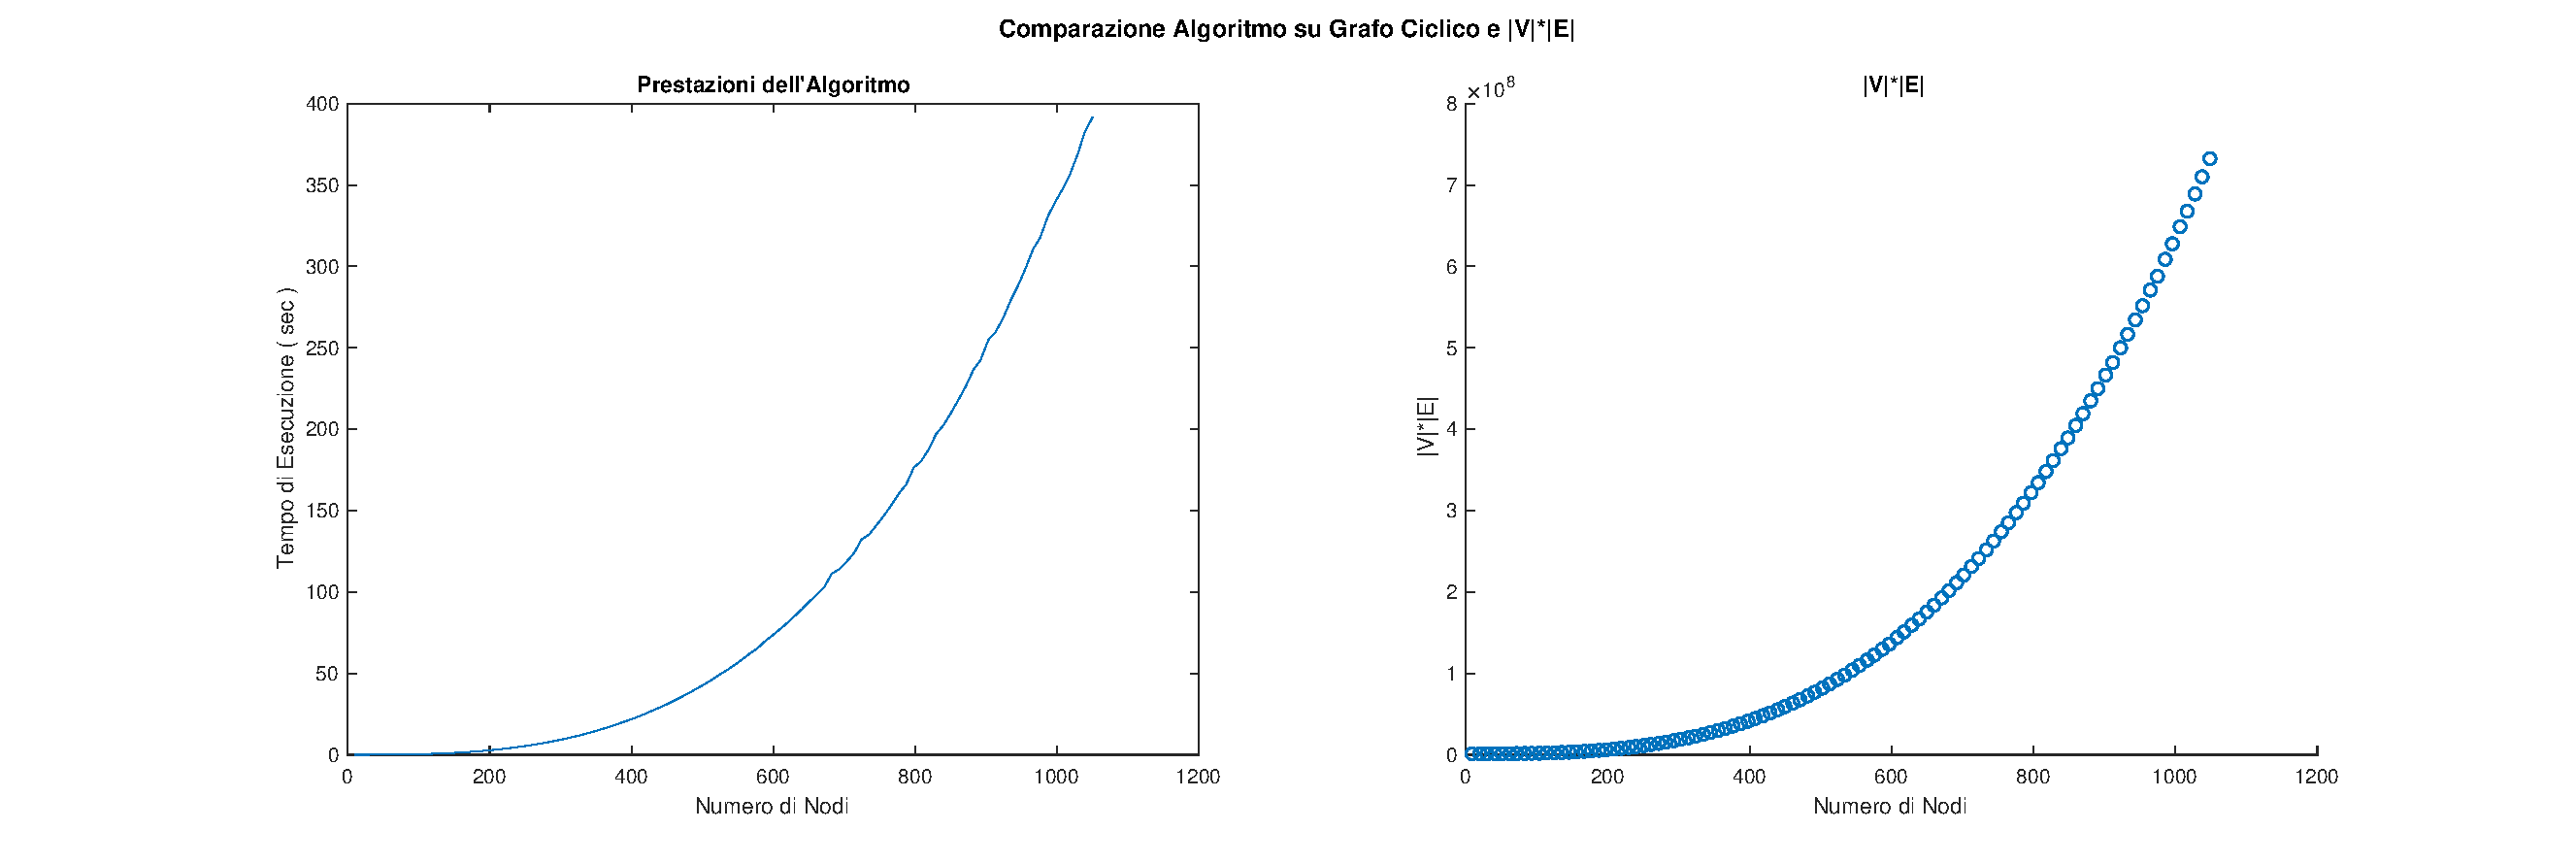
\includegraphics[width=\textwidth,height=\textheight,keepaspectratio]{./TeX_files/chart/Ciclico}
    \caption{Grafico che mette a confronto numero di nodi/tempo di esecuzione e  numero di nodi/$|V|*|E|$ per grafi Ciclici}
\vspace{-10pt}
\end{figure}

\begin{figure}[H]
	\vspace{-10pt}
	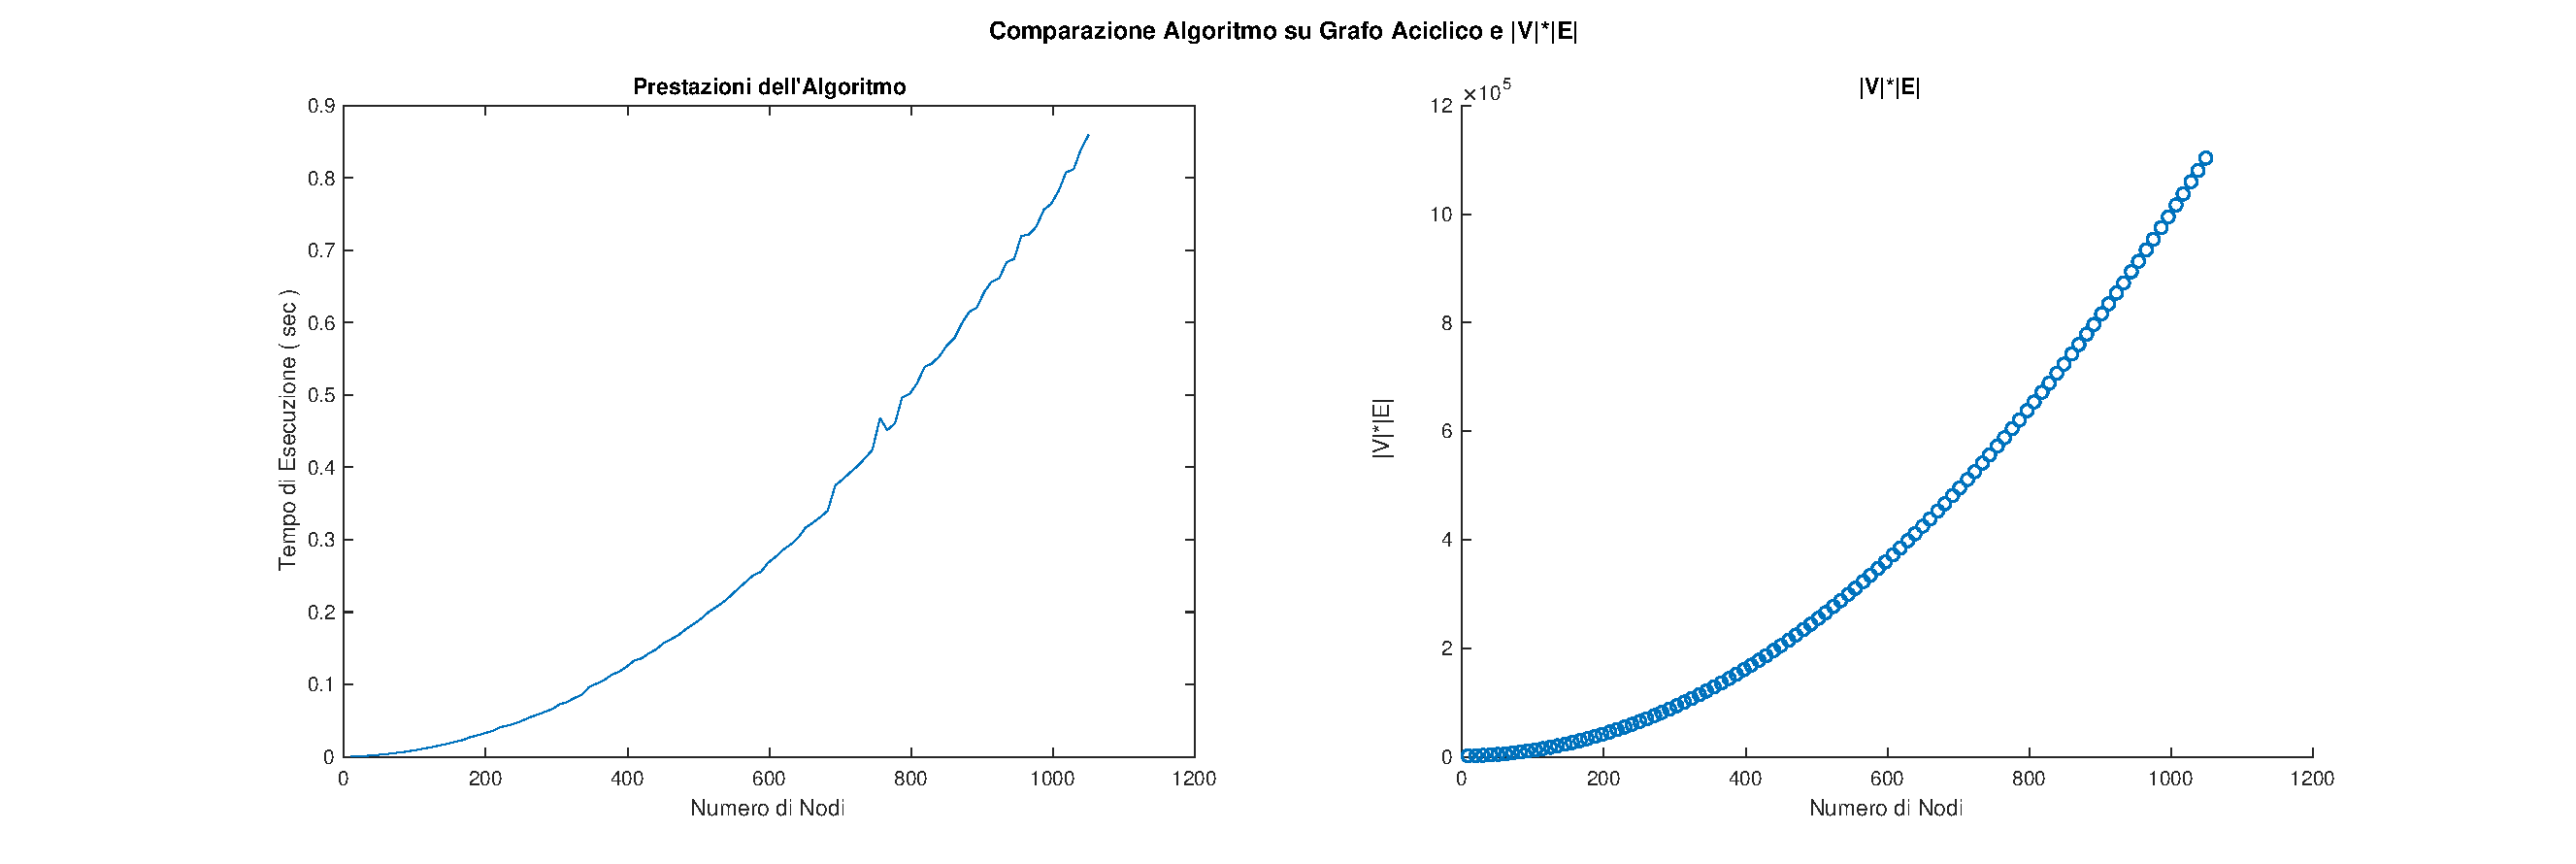
\includegraphics[width=\textwidth,height=\textheight,keepaspectratio]{./TeX_files/chart/Aciclico}
	\caption{Grafico che mette a confronto numero di nodi/tempo di esecuzione e  numero di nodi/$|V|*|E|$ per grafi Aciclici}
	\vspace{-10pt}
\end{figure}

\noindent Come si evince dalle Figure 4.1-2, la complessità temporale studiata teoricamente nell'analisi teorica dell'algoritmo è risultata corretta e supportata da evidenze sperimentali. Data una ricerca più approfondita in materia, l'algoritmo di Brandes detiene tutt'ora adesso il "primato" ( se pur nel recente periodo sia stato ampliato e ancora più raffinato ), pur essendo un algoritmo di carattere statico e avendo validissimi algoritmi di tipologia euristica come avversari. La peculiarità del presente algoritmo è insita nella "intrinseca parallelità". É infatti possibile modificare l'algoritmo e adattarlo ad una tipologia di approccio clusteristico nel quale si può demandare il calcolo dei cammini minimi e delle dipendenze a diversi core di elaborazione e quindi eseguire il tutto in parallelo.


\chapter{Bibliografia}
\section{L'Algoritmo di Brandes}
	\emph{"L'indice di Betweenness Centrality  è essenziale nell'analisi dei social network, ma costoso da calcolare. Attualmente, gli algoritmi più veloci richiedono tempo $\Theta(n^3)$ e spazio $\Theta(n^2)$, dove n è il numero di attori nella rete. Motivati dalla crescente necessità di calcolare gli indici di Betweenness Centrality su reti grandi ma molto sparse, in questo articolo vengono introdotti nuovi algoritmi per le relazioni interpersonali. Richiedono spazio $O(n + m)$ ed eseguono la richiesta in tempo $O(nm)$ e $O(nm + n^2log(n))$ su grafi pesati e non, rispettivamente, dove m è il numero di collegamenti "}\\ 
\begin{flushright}
 -Abstract, A Faster Algorithm for Betweenness Centrality, Ulrik Brandes\\
\end{flushright}

\noindent Avendo identificato nel problema postoci la possibilità che tale argomento fosse di largo interesse, mi sono tuffato nella ricerca di paper accademici e dopo un po di \emph{"digging"} nella rete ho scoperto questo Paper Accademico dal titolo \emph{A Faster Algorithm for Betweenness Centrality} del prof. Ulrik Brandes.Nel suo approfondire lo stesso, mi sono reso conto della rilevanza di tale algoritmo e dei risultati sperimentali e reali che questo algoritmo ha registrato nonché della sua stessa incidenza sull'analisi di grafi più complessi dato il ridotto "time" di esecuzione.
Il Paper, liberamente fruibile dalla rete, è stato comunque inserito nella cartella "Papers" del progetto al fine di fornire subito la reference in "locale" inoltre, sono stati accennati difatti alcuni risultati come l'ormai "famoso" Corollario 4, che dimostra senza alcun dubbio come il calcolo delle dipendenze e dei cammini minimi possa essere portato a termine con una Complessità Temporale pari a $O(m)$
\\Il Paper è stato pubblicato per la prima volta in \emph{Journal of Mathematical Sociology 25(2):163-177, (2001).}
\chapter{Conclusione}
\section{Riflessioni Finali}
L'interezza dell'algoritmo è stata così presentata in questa "breve" relazione. Al fine di aiutare nella comprensione del codice e della relazione stessa ho scritto effettivamente alcune funzioni sovrabbondati rispetto al codice fornitoci dai tutor, magari sprecato memoria nella creazione di un grafo temporaneo od omesso alcuni passaggi di secondaria importanza dell'algoritmo in questa stessa relazione, tali scelte però sono state dettate da una criterio puramente "didattico" per aiutare nella migliore comprensione del codice.
Lavorare su questo progetto è stato davvero un piacere non solo di carattere puramente esercitativo bensì scientifico. Per risolvere il problema di Betweennes Centrality ho avuto la possibilità di ricercare nei Papers Accademici e ciò è stato davvero edificante. Molto curioso ed interessante, quindi degno di nota, è il differente Tempo di Esecuzione tra grafi Ciclici ed Aciclici, tale divario poteva essere stimato come marginale invece è stato davvero rilevante ( 0.85 per 1050 nodi aciclici mentre circa circa 4 minuti per i ciclici ).
\\
Tutto il codice è rilasciato sotto la MIT License. 
\begin{flushright}
	\emph{Matteo Esposito}
\end{flushright}

%--------------------------------------%

\backmatter
\end{document}